\section{Ripasso Proprietà Variabili Aleatorie}\label{sec:ripasso_va}

\subsection{Definizioni Generali}\label{ssec:def_generali}
Ripassiamo i concetti fondamentali di Funzione di Ripartizione Cumulativa (CDF), Funzione di Densità di Probabilità (PDF) per variabili continue, e Funzione di Massa di Probabilità (PMF) per variabili discrete.

\begin{definizione}{Funzione di Ripartizione Cumulativa (CDF)}{cdf}
La CDF, indicata con \( F_X(t) \), descrive la probabilità che una variabile aleatoria (v.a.) \( X \) assuma un valore minore o uguale a \( t \).
\[
F_X(t) = P(X \le t)
\]
La CDF è una funzione non decrescente con valori compresi tra 0 e 1. Per una v.a. continua, la CDF è una funzione continua, mentre per una v.a. discreta è una funzione a gradini.
\end{definizione}

\begin{definizione}{PDF (per v.a. continue) e PMF (per v.a. discrete)}{pdf_pmf}
\begin{itemize}
    \item La \textbf{Funzione di Densità di Probabilità (PDF)}, \( f(t) \), per una v.a. continua, è la derivata della CDF. L'area sottesa alla curva della PDF tra due punti \( a \) e \( b \) rappresenta la probabilità che la variabile cada in quell'intervallo.
    \[
    f(t) = F'(t) \quad \text{e} \quad P(a < X \le b) = \int_a^b f(t) \,dt = F(b) - F(a)
    \]
    \item La \textbf{Funzione di Massa di Probabilità (PMF)}, \( \varphi_X(k) \), per una v.a. discreta, dà la probabilità esatta che la variabile assuma il valore \( k \).
    \[
    \varphi_X(k) = P(X = k) = F_X(k) - F_X(k-1)
    \]
    La CDF può essere ottenuta sommando i valori della PMF.
    \[
    F_X(k) = \sum_{j \le k} \varphi_X(j)
    \]
\end{itemize}
\end{definizione}

\begin{nota}{Calcolo di probabilità tramite CDF}{calcolo_prob}
Ecco un riassunto delle formule per calcolare la probabilità di un evento usando la CDF:
\begin{itemize}
    \item \textbf{Coda sinistra (v.a. continue e discrete):} Probabilità che \( X \) sia minore o uguale ad \( a \).
    \[ P(X \le a) = F_X(a) \]
    \item \textbf{Coda destra (v.a. continue):} Probabilità che \( X \) sia maggiore di \( b \).
    \[ P(X > b) = 1 - F_X(b) \]
    \item \textbf{Coda destra (v.a. discrete):} Probabilità che \( X \) sia maggiore o uguale a \( b \).
    \[ P(X \ge b) = 1 - F_X(b-1) \]
    \item \textbf{Intervallo (v.a. continue):} Probabilità che \( X \) sia compreso tra \( a \) e \( b \).
    \[ P(a < X \le b) = F_X(b) - F_X(a) \]
    \item \textbf{Intervallo (v.a. discrete, estremi esclusi):} Probabilità che \( X \) sia strettamente compreso tra \( a \) e \( b \).
    \[ P(a < X < b) = P(X \le b-1) - P(X \le a) = F_X(b-1) - F_X(a) \]
\end{itemize}
\end{nota}

\subsection{Inversione della Formula}\label{ssec:inversione}

Un uso molto comune della CDF è il calcolo del \textbf{quantile}, ovvero l'inversione della formula per trovare il valore \( x \) corrispondente a una data probabilità cumulata.

\begin{nota}{Quantile}{quantile}
Il \textbf{quantile} di livello \(p \in (0,1)\) di una variabile aleatoria \(X\) è il valore soglia \(q_p\) tale che:
\[
P(X \leq q_p) = p.
\]
In altre parole, il quantile è l’inversa della funzione di ripartizione cumulativa (CDF): 
\[
q_p = F_X^{-1}(p).
\]
Esempi importanti sono la \textit{mediana} (\(p=0.5\)), i \textit{quartili} (\(p=0.25,0.75\)) e in generale i \textit{percentili}. 
Essi permettono di descrivere in modo sintetico la distribuzione di una variabile e sono usati in statistica descrittiva, test d’ipotesi e intervalli di confidenza.
\end{nota}
\begin{esempio}{Trovare un quantile da una probabilità}{inversione_gamma}
Supponiamo di voler trovare il valore \( x \) per cui la probabilità che una variabile con distribuzione Gamma \( \gamma(\alpha, \beta) \) sia minore o uguale a \( x \) sia almeno del 5\%.
\begin{enumerate}
    \item \textbf{Impostare la disequazione:}
    \[
    P(\text{gamma}(\alpha, \beta) \le x) \ge 0.05
    \]
    \item \textbf{Esprimere tramite CDF:}
    \[
    F_{\text{gamma}}(x) \ge 0.05
    \]
    \item \textbf{Applicare la funzione inversa della CDF ($F_g^{-1}$):} Poiché la CDF e la sua inversa sono funzioni crescenti, il verso della disuguaglianza non cambia.
    \[
    F_g^{-1}(F_g(x)) \ge F_g^{-1}(0.05)
    \]
    \item \textbf{Risolvere per \(x\):}
    \[
    x \ge F_g^{-1}(0.05)
    \]
\end{enumerate}
La conclusione è che tutti i valori di \( x \) maggiori o uguali al quantile al 5\% della distribuzione Gamma soddisfano la richiesta. In software come Excel, questo valore si calcola con la funzione \texttt{GAMMA.INV(0.05, alpha, beta)}.
\end{esempio}

\subsection{Inversione con Due Incognite}\label{ssec:inversione_due_incognite}
Spesso si cerca un intervallo \( [a, b] \) tale per cui la probabilità che una variabile aleatoria cada al suo interno sia pari a un valore prefissato (es. 90\% o 95\%), tipicamente per costruire intervalli di confidenza.
\[
P(X \in [a, b]) = 1 - \alpha
\]
Ad esempio, se vogliamo \( P(a \le X \le b) = 90\% \), la probabilità totale nelle code (a sinistra di \(a\) e a destra di \(b\)) deve essere del 10\%. Poiché ci sono infinite coppie \( (a, b) \) che soddisfano questa condizione, si usano dei criteri per scegliere una soluzione unica.

\begin{nota}{Criteri per la scelta dell'intervallo}{criteri_intervallo}
I tre criteri più comuni sono:
\begin{itemize}
    \item \textbf{Intervallo Canonico (o delle code uguali):} La probabilità residua \( \alpha \) viene divisa equamente tra le due code. Se \( \alpha = 10\% \), si pone il 5\% sulla coda sinistra e il 5\% sulla destra.
    \[
    a = F_X^{-1}(0.05) \quad \text{e} \quad b = F_X^{-1}(0.95)
    \]
    \item \textbf{Intervallo Arbitrario:} La probabilità \( \alpha \) viene suddivisa in modo arbitrario, purché la somma sia corretta. Ad esempio, si potrebbe avere una coda sinistra con il 7\% di probabilità e una destra con il 3\%.
    \item \textbf{Intervallo di ampiezza minima:} Si cerca l'intervallo \( [a, b] \) che, a parità di probabilità interna, ha la larghezza \( (b-a) \) più piccola possibile. Per una distribuzione unimodale continua, questo si ottiene quando la funzione di densità ha la stessa altezza agli estremi.
    \[
    f(a) = f(b)
    \]
\end{itemize}
\end{nota}

\begin{nota}{Caso delle distribuzioni simmetriche}{intervallo_simmetrico}
Se la distribuzione di probabilità è simmetrica e unimodale (es. Normale, t di Student), l'intervallo \textbf{canonico} (a code uguali) coincide con l'intervallo di \textbf{ampiezza minima}.
\end{nota}

\subsection{Proprietà di Simmetria e Correzione per la Continuità}

\begin{nota}{Simmetria della CDF per distribuzioni simmetriche}{simmetria_cdf}
Per una distribuzione simmetrica attorno a zero, come la Normale standard \( \mathcal{N}(0,1) \), la CDF \( \Phi(x) \) ha le seguenti proprietà:
\[
\Phi(-x) = 1 - \Phi(x) \implies \Phi(x) + \Phi(-x) = 1
\]
Questa proprietà si estende anche alla sua funzione inversa (la funzione quantile):
\[
\Phi^{-1}(\alpha) = - \Phi^{-1}(1-\alpha)
\]
Ciò significa che il quantile di livello \( \alpha \) è l'opposto del quantile di livello \( 1-\alpha \).
\end{nota}

\begin{nota}{Correzione per la Continuità}{correzione_continuita}
Quando si approssima una v.a. discreta (che assume valori interi) con una v.a. continua, si introduce un errore. La \textbf{correzione per la continuità} serve a ridurre questo errore.
Per calcolare \( P(X \le k) \) dove \( X \) è una v.a. discreta, usando la CDF continua \( F \) come approssimazione, è più accurato calcolare \( F \) nel punto \( k+0.5 \).
\[
F_X(k) = P(X_{\text{discreta}} \le k) \approx F_{\text{continua}}(k + 0.5)
\]
Questo perché \( k+0.5 \) è il punto medio tra \(k\) e \(k+1\), fornendo una stima migliore del valore della funzione a gradini discreta.
\end{nota}

\subsection{Generazione di v.a. con Legge Data}\label{ssec:generazione_va}
Il metodo dell'\textbf{Inverse Transform Sampling} (Campionamento tramite Inversione della Trasformata) permette di generare numeri casuali da qualsiasi distribuzione di probabilità di cui sia nota la CDF. Si basa sulla trasformazione integrale di probabilità.

\begin{proposizione}{Metodo dell'Inverse Transform Sampling}{its}
Sia \( F \) la CDF di una distribuzione target. Per generare un campione \( X \) da questa distribuzione:
\begin{enumerate}
    \item Si genera un numero casuale \( U \) da una distribuzione Uniforme in \( [0, 1] \).
    \item Si calcola \( X = F^{-1}(U) \), dove \( F^{-1} \) è la funzione quantile (l'inversa della CDF).
\end{enumerate}
La variabile aleatoria \( X \) così generata avrà come distribuzione proprio quella descritta da \( F \).
\end{proposizione}

\begin{esempio}{Generazione da una distribuzione Esponenziale}{gen_exp}
Vogliamo generare un campione da una distribuzione Esponenziale di parametro \( \lambda \).
\begin{enumerate}
    \item \textbf{CDF:} \( F(t) = 1 - e^{-\lambda t} \) per \( t \ge 0 \).
    \item \textbf{Inversa della CDF:} Poniamo \( y = 1 - e^{-\lambda t} \) e risolviamo per \( t \).
    \[
    1-y = e^{-\lambda t} \implies \log(1-y) = -\lambda t \implies t = -\frac{1}{\lambda}\log(1-y)
    \]
    Quindi \( F^{-1}(y) = -\frac{1}{\lambda}\log(1-y) \).
    \item \textbf{Generazione:} Generiamo \( U \sim \text{Unif}(0,1) \) e calcoliamo:
    \[
    X = F^{-1}(U) = -\frac{1}{\lambda}\log(1-U)
    \]
\end{enumerate}
\end{esempio}

\begin{dimostrazione}{Giustificazione del metodo}{its}
Vogliamo dimostrare che la CDF di \( X = F^{-1}(U) \) è proprio \( F \). Sia \( F_X(t) \) la CDF di \( X \).
\[
F_X(t) = P(X \le t) = P(F^{-1}(U) \le t)
\]
Poiché \( F \) è una funzione crescente, possiamo applicarla a entrambi i lati della disuguaglianza senza cambiarne il verso:
\[
P(F^{-1}(U) \le t) = P(U \le F(t))
\]
Dato che \( U \sim \text{Unif}(0,1) \), per definizione la sua CDF è \( F_U(y) = P(U \le y) = y \). Sostituendo \( y = F(t) \), otteniamo:
\[
P(U \le F(t)) = F(t)
\]
Abbiamo quindi dimostrato che \( F_X(t) = F(t) \), confermando che la variabile \( X \) generata ha la distribuzione desiderata.
\end{dimostrazione}

\subsection{CDF Empirica e Diagramma Q-Q}\label{ssec:ecdf_qq}
Quando non si conosce la vera distribuzione di un set di dati, si possono usare strumenti empirici per stimarla e visualizzarla.

\begin{definizione}{Funzione di Ripartizione Cumulativa Empirica (ECDF)}{ecdf}
Dato un campione di \( n \) osservazioni \( x_1, \dots, x_n \), la \textbf{CDF Empirica} \( \hat{F}_n(t) \) è la proporzione di osservazioni nel campione che sono minori o uguali a \( t \).
\[
\hat{F}_n(t) = \frac{\#\{i: x_i \le t\}}{n}
\]
Graficamente, è una funzione a gradini che aumenta di \( 1/n \) in corrispondenza di ogni dato osservato. La ECDF è una stima della vera CDF (sconosciuta) della popolazione da cui il campione è stato estratto.
\end{definizione}

\paragraph{Diagramma Q-Q (Quantile-Quantile)}
Il diagramma Q-Q è uno degli strumenti grafici più efficaci per confrontare la distribuzione dei dati con una distribuzione teorica. L'idea è quella di plottare i quantili campionari (i dati ordinati) contro i quantili teorici della distribuzione di riferimento.

Se i dati seguono la distribuzione teorica, i punti sul grafico si allineano lungo una retta. Per verificare l'ipotesi di normalità (o gaussianità), si costruisce il grafico plottando i punti:
\[
\left( \Phi^{-1}\left( \frac{i-0.5}{n} \right), x_{(i)} \right)
\]
dove \( x_{(i)} \) è l'i-esimo dato ordinato e \( \Phi^{-1} \) è la funzione quantile della Normale standard.

\begin{nota}{Derivazione Matematica e Interpretazione}{qq_plot_logic}
La linearità del grafico Q-Q per dati Normali deriva da una relazione matematica precisa.

\paragraph{Relazione Fondamentale.}
Supponiamo che i nostri dati \( x_i \) seguano una distribuzione Normale \( \mathcal{N}(\mu, \sigma^2) \). Allora, ogni punto può essere espresso in termini di un quantile \( p_i \) e della funzione quantile inversa della Normale standard, \( \Phi^{-1} \).
\[
p_i = \Phi\left(\frac{x_i - \mu}{\sigma}\right) \iff x_i = \mu + \sigma \Phi^{-1}(p_i)
\]
Questa equazione mostra che ogni quantile dei nostri dati, \( x_i \), è una funzione lineare del quantile corrispondente di una Normale standard, \( \Phi^{-1}(p_i) \).

\paragraph{Costruzione del Grafico.}
Per costruire il grafico, confrontiamo i quantili campionari (i nostri dati ordinati) con i quantili teorici.
\begin{itemize}
    \item \textbf{Asse Y (Quantili Campionari):} Utilizziamo i dati osservati e ordinati: \[ x_{(1)}, x_{(2)}, \dots, x_{(n)} \]
    \item \textbf{Asse X (Quantili Teorici):} Dobbiamo calcolare i quantili teorici corrispondenti. Se i dati fossero Normali, le probabilità cumulate \( p_{(i)} \) associate a ogni \( x_{(i)} \) sarebbero uniformemente distribuite. Approssimiamo queste probabilità con le posizioni di plotting:
    \[
    p_{(i)} \approx \frac{i-0.5}{n}, \quad \text{per } i=1, \dots, n
    \]
    I quantili teorici della Normale standard sono quindi:
    \[
    z_i = \Phi^{-1}\left( \frac{i-0.5}{n} \right)
    \]
\end{itemize}

\paragraph{Interpretazione.}
Il diagramma Q-Q plotta i punti \( (z_i, x_{(i)}) \). Se l'ipotesi di normalità è vera, allora, sostituendo nell'equazione fondamentale, otteniamo:
\[
x_{(i)} \approx \mu + \sigma \Phi^{-1}(p_{(i)}) \approx \mu + \sigma z_i
\]
I punti del grafico \( (z_i, x_{(i)}) \) dovrebbero quindi giacere approssimativamente sulla retta \( y = \mu + \sigma z \). Una deviazione sistematica da questa retta indica che i dati non seguono una distribuzione Normale.
\end{nota}

\section{Leggi di Variabili Aleatorie Importanti}\label{sec:leggi_va}

\subsection{Distribuzione Gaussiana (o Normale)}
La distribuzione Gaussiana è una delle più importanti in statistica, descrivendo molti fenomeni naturali che risultano dalla somma di numerosi piccoli effetti indipendenti.

\begin{definizione}{Distribuzione Gaussiana}{gaussiana}
Una variabile aleatoria \(X\) segue una distribuzione Gaussiana con media \(\mu\) e varianza \(\sigma^2\), indicata con \(X \sim \mathcal{N}(\mu, \sigma^2)\), se la sua funzione di densità di probabilità (PDF) è:
\[
f(x) = \frac{1}{\sqrt{2\pi\sigma^2}} \exp\left\{ -\frac{(x-\mu)^2}{2\sigma^2} \right\}, \quad x \in \mathbb{R}
\]

\end{definizione}

\begin{nota}{Teorema del Limite Centrale (TLC)}{tlc}
Il TLC afferma che le grandezze casuali che sono la \textbf{somma} di tanti piccoli contributi indipendenti tendono ad avere una distribuzione Normale.
\end{nota}

\begin{proposizione}{Proprietà della Gaussiana}{gauss_props}
\begin{itemize}
    \item \textbf{Chiusura per trasformazioni lineari:} Se \(X \sim \mathcal{N}(\mu, \sigma^2)\), allora la trasformazione lineare \(a + bX\) segue ancora una distribuzione Normale:
    \[ a+bX \sim \mathcal{N}(a+b\mu, b^2\sigma^2) \]
    \item \textbf{Riproducibilità:} La somma di due v.a. Gaussiane \emph{indipendenti} è ancora una v.a. Gaussiana. Se \(X \sim \mathcal{N}(\mu_1, \sigma_1^2)\) e \(Y \sim \mathcal{N}(\mu_2, \sigma_2^2)\) sono indipendenti:
    \[ X+Y \sim \mathcal{N}(\mu_1+\mu_2, \sigma_1^2+\sigma_2^2) \]
    \item \textbf{CDF Canonica:} La CDF di una qualsiasi Normale può essere ricondotta a quella della Normale standard \( \Phi(t) = F_{\mathcal{N}(0,1)}(t) \):
    \[ F_{\mathcal{N}(\mu,\sigma^2)}(x) = P(X \le x) = \Phi\left(\frac{x-\mu}{\sigma}\right) \]
\end{itemize}
\end{proposizione}

\begin{figure}[H]
    \centering
    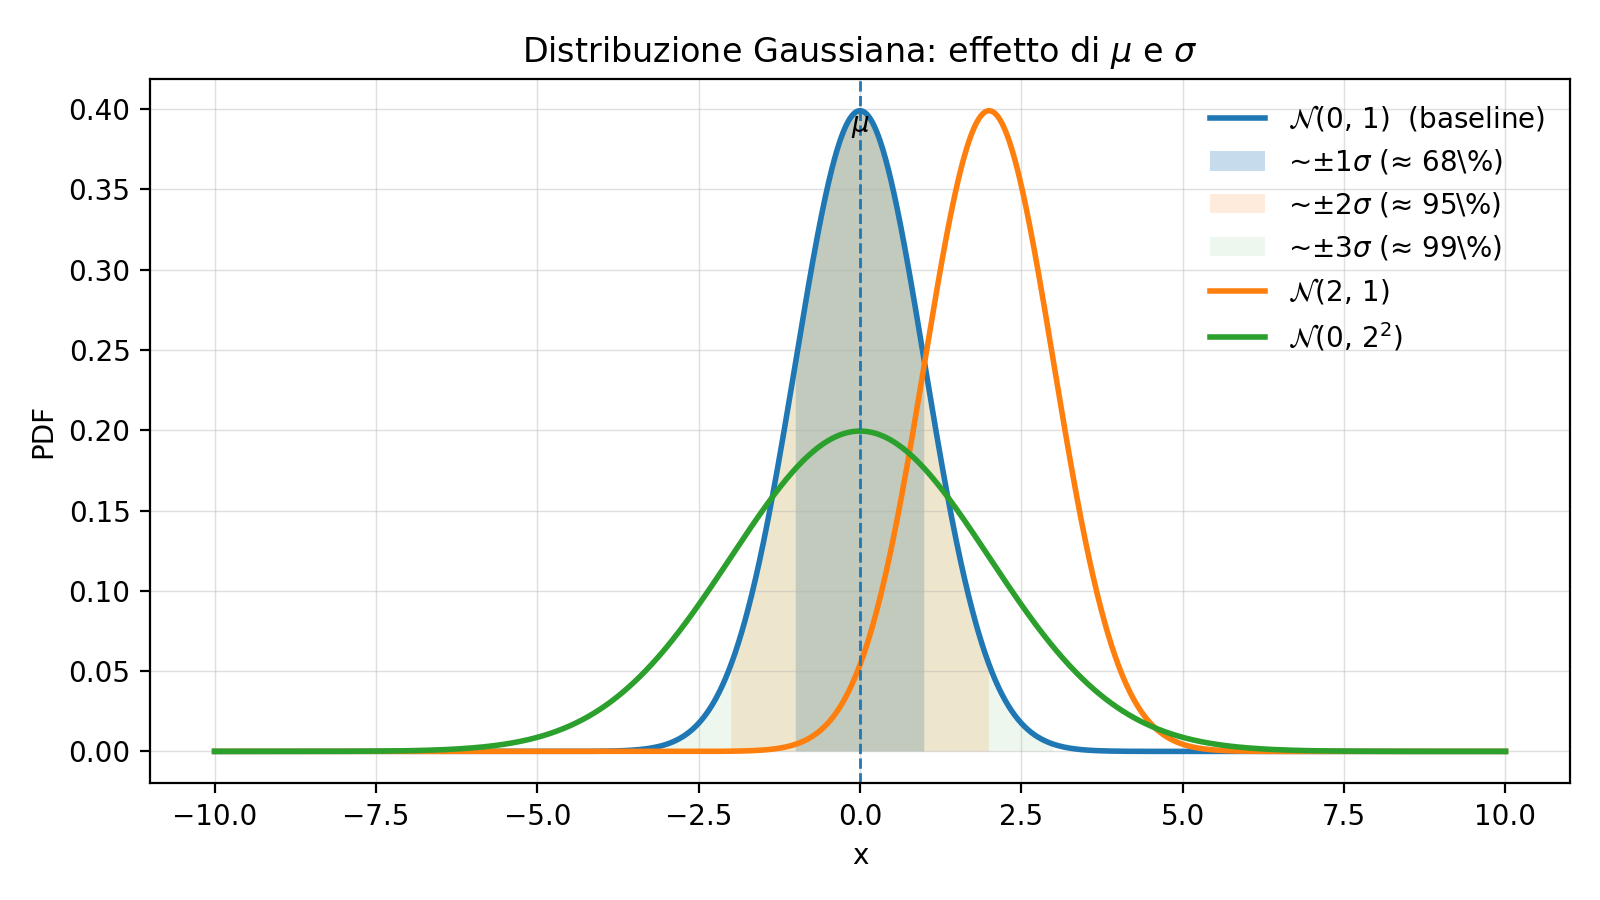
\includegraphics[width=0.8\textwidth]{images/gaussiana.png}
    \caption{Esempio di distribuzioni Gaussiane con \(\mu=0\) e \(\sigma\) variabile.}
    \label{fig:gaussiana}
\end{figure}

\subsection{Distribuzione Lognormale}
La Lognormale descrive grandezze che derivano dal \emph{prodotto} di molti fattori casuali.

\begin{definizione}{Distribuzione Lognormale}{lognormale}
Una variabile aleatoria \(X\) è Lognormale se il suo logaritmo naturale è una v.a. Normale. Se \(Y = \log X \sim \mathcal{N}(\mu, \sigma^2)\), allora si scrive \(X \sim \text{Lognorm}(\mu, \sigma^2)\). In altre parole, è l'esponenziale di una Gaussiana:
\[ X = e^Y, \quad \text{con } Y \sim \mathcal{N}(\mu, \sigma^2) \]
\end{definizione}

\begin{nota}{Origine della Lognormale}{lognorm_origin}
Una versione "moltiplicativa" del TLC afferma che le grandezze che sono il \textbf{prodotto} di tanti piccoli contributi indipendenti tendono ad avere una distribuzione Lognormale. Esempi tipici sono redditi, patrimoni e dimensioni di frammenti.
\end{nota}

\begin{proposizione}{Proprietà della Lognormale}{lognorm_props}
\begin{itemize}
    \item \textbf{Asimmetria:} È una distribuzione asimmetrica con una coda lunga a destra, adatta a modellare quantità che non possono essere negative ma possono assumere valori molto grandi.
    \item \textbf{Analisi dei dati:} Per analizzare dati lognormali, è pratica comune calcolarne il logaritmo e trattare i dati trasformati come Normali.
    \item \textbf{Media e Mediana:} A differenza della Normale, media e mediana non coincidono.
    \[ E(X) = e^{\mu + \frac{\sigma^2}{2}}, \quad \text{Mediana}(X) = e^\mu \]
\end{itemize}
\end{proposizione}

\begin{figure}[H]
    \centering
    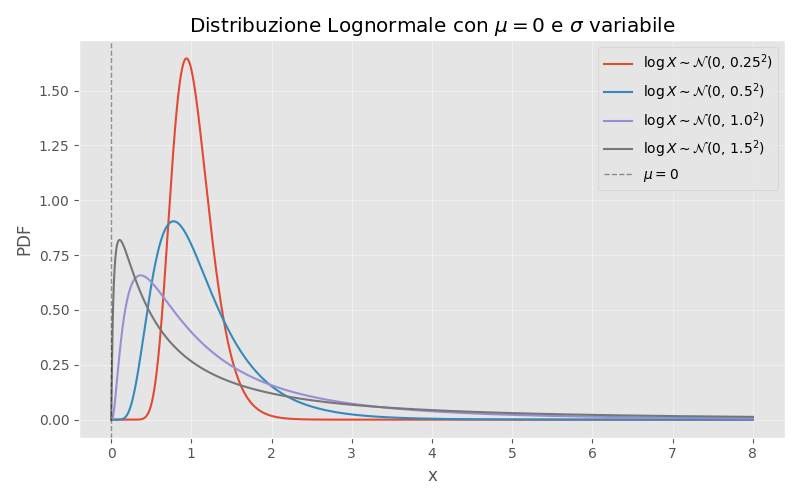
\includegraphics[width=0.8\textwidth]{images/lognormale.png}
    \caption{Esempio di distribuzioni Lognormali con \(\mu=0\) e \(\sigma\) variabile.}
    \label{fig:lognormale}
\end{figure}

\subsection{Distribuzione Esponenziale}
L'Esponenziale è la distribuzione di base per i tempi di attesa.

\begin{definizione}{Distribuzione Esponenziale}{esponenziale}
Una v.a. \(T\) segue una distribuzione Esponenziale di parametro \(\lambda > 0\), indicata con \(T \sim \text{Expo}(\lambda)\), se la sua PDF è:
\[
f_T(t) = \lambda e^{-\lambda t}, \quad t \ge 0
\]
Il parametro \(\lambda\) è chiamato \textbf{tasso} o \textbf{intensità}, e rappresenta il numero medio di eventi nell'unità di tempo.
\end{definizione}

\begin{proposizione}{Proprietà dell'Esponenziale}{expo_props}
\begin{itemize}
    \item \textbf{Versione continua della Geometrica:} Rappresenta il tempo di attesa per un evento che ha la stessa "probabilità" infinitesima di avvenire in ogni istante.
    \item \textbf{Assenza di memoria:} La probabilità di attendere ancora non dipende da quanto si è già atteso. Formalmente:
    \[ P(T > a+b \mid T > a) = P(T > b) \]
    \item \textbf{Applicazioni:} Modella tempi di attesa per eventi improvvisi e imprevedibili come guasti, telefonate, decadimenti radioattivi.
\end{itemize}
\end{proposizione}

\begin{figure}[H]
    \centering
    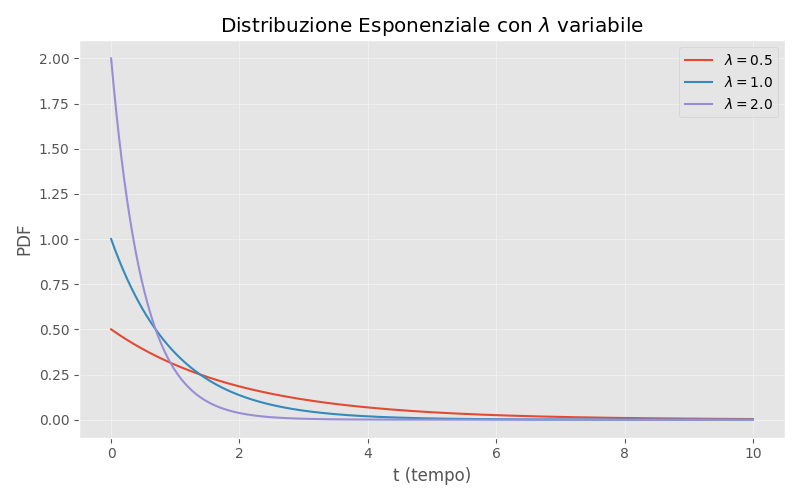
\includegraphics[width=0.8\textwidth]{images/esponenziale.png}
    \caption{Esempio di distribuzioni Esponenziali con \(\lambda\) variabile.}
    \label{fig:esponenziale}
\end{figure}

\subsection{Distribuzione Gamma}
La distribuzione Gamma è una generalizzazione dell'Esponenziale e della Chi-Quadro, molto flessibile per modellare tempi di attesa.

\begin{definizione}{Distribuzione Gamma}{gamma}
Una v.a. \(X\) segue una distribuzione Gamma definita da un parametro di forma \(\alpha>0\) e un parametro di tasso \(\lambda>0\). Si indica \(X \sim \text{Gamma}(\alpha, \lambda)\). La sua PDF è:
\[
f(t) = \frac{\lambda^\alpha}{\Gamma(\alpha)} t^{\alpha-1} e^{-\lambda t}, \quad t>0
\]
dove \(\Gamma(\alpha)\) è la funzione Gamma di Eulero. Una parametrizzazione alternativa usa un parametro di scala \(\beta = 1/\lambda\).
\end{definizione}

\begin{proposizione}{Proprietà della Gamma}{gamma_props}
\begin{itemize}
    \item \textbf{Riproducibilità:} La somma di v.a. Gamma indipendenti con lo stesso tasso \(\lambda\) è ancora una Gamma. Se \(X \sim \text{Gamma}(\alpha_1, \lambda)\) e \(Y \sim \text{Gamma}(\alpha_2, \lambda)\) sono indipendenti:
    \[ X+Y \sim \text{Gamma}(\alpha_1+\alpha_2, \lambda) \]
    \item \textbf{Scalatura:} Se \(X \sim \text{Gamma}(\alpha, \lambda)\), allora \(cX \sim \text{Gamma}(\alpha, \lambda/c)\).
    \item \textbf{Media e Varianza:}
    \[ E(X) = \frac{\alpha}{\lambda}, \quad \text{Var}(X) = \frac{\alpha}{\lambda^2} \]
\end{itemize}
\end{proposizione}

\begin{figure}[H]
    \centering
    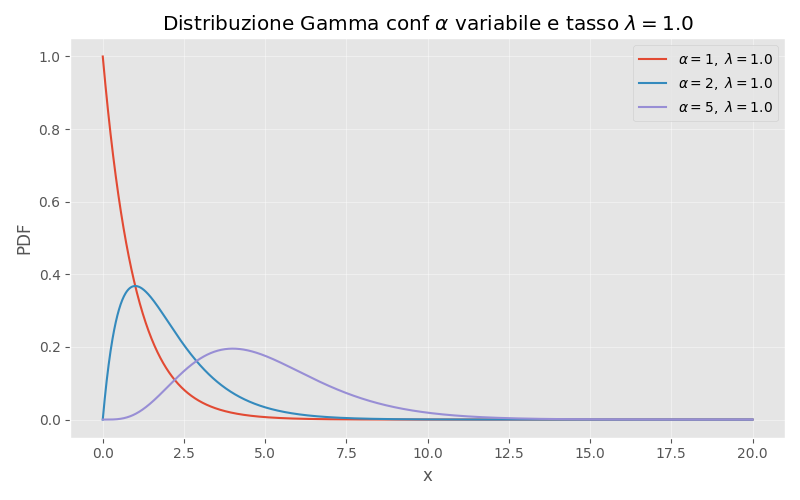
\includegraphics[width=0.8\textwidth]{images/gamma.png}
    \caption{Esempio di distribuzioni Gamma con \(\alpha\) variabili e \(\lambda\) costante.}
    \label{fig:gamma}
\end{figure}

\begin{nota}{Casi Particolari della Gamma}{gamma_casi}
\begin{itemize}
    \item \textbf{Esponenziale:} Per \(\alpha=1\), la Gamma diventa un'Esponenziale: \(\text{Gamma}(1, \lambda) \equiv \text{Expo}(\lambda)\).
    \item \textbf{Erlang:} Se \(\alpha=n\) è un intero, la distribuzione si chiama Erlang ed è la somma di \(n\) v.a. \(\text{Expo}(\lambda)\) indipendenti.
    \item \textbf{Chi-Quadro:} È un altro caso speciale, fondamentale in statistica.
\end{itemize}
\end{nota}

\subsection{Distribuzione Chi-Quadro}
\begin{definizione}{Distribuzione Chi-Quadro}{chi_quadro}
Una v.a. \(W\) segue una distribuzione Chi-Quadro con \(k\) gradi di libertà, \(W \sim \chi^2(k)\), se è la somma dei quadrati di \(k\) v.a. Normali standard indipendenti.
\[
W = \sum_{i=1}^k Z_i^2, \quad \text{dove } Z_i \sim \mathcal{N}(0,1) \text{ i.i.d.}
\]
È un caso particolare della Gamma: \( \chi^2(k) \equiv \text{Gamma}(k/2, 1/2) \).
\end{definizione}

\begin{nota}{Proprietà della Chi-Quadro}{chi_props}
Derivando dalla Gamma, si ottiene:
\[ E(W) = k, \quad \text{Var}(W) = 2k \]
Inoltre, poiché \( Z^2 \sim \chi^2(1) \), si ha che \(\chi^2(1) \equiv \text{Gamma}(1/2, 1/2)\).
\end{nota}

\begin{figure}[H]
    \centering
    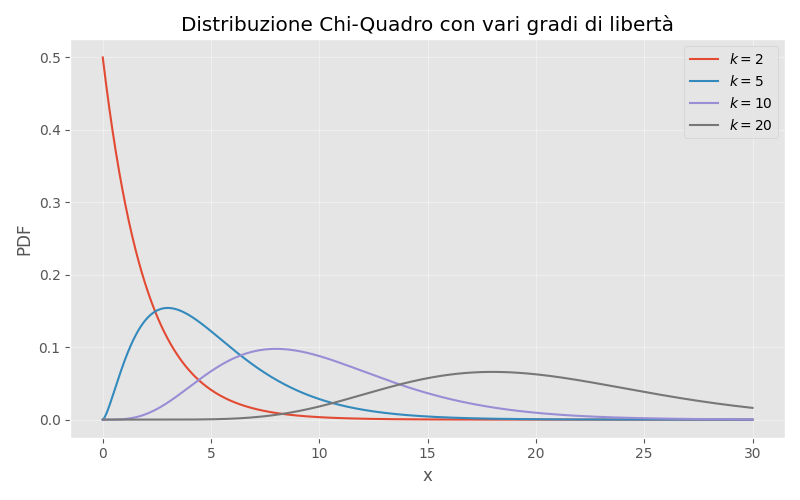
\includegraphics[width=0.8\textwidth]{images/chi2.png}
    \caption{Esempio di distribuzioni Chi-Quadro con \(k\) variabili.}
    \label{fig:chi2}
\end{figure}

\subsection{Il Processo di Poisson}
Il processo di Poisson descrive il verificarsi di eventi casuali nel tempo.

\begin{definizione}{Processo di Poisson}{poisson_proc}
Un processo di Poisson è una sequenza di eventi istantanei tali che i tempi di inter-arrivo tra un evento e il successivo sono variabili aleatorie indipendenti e identicamente distribuite (i.i.d.) come un'Esponenziale di tasso \(\lambda\).
\end{definizione}

\begin{proposizione}{Componenti del Processo di Poisson}{poisson_comp}
\begin{itemize}
    \item \textbf{Tempi di inter-arrivo \(T_i\):} Il tempo tra l'evento \(i-1\) e l'evento \(i\).
    \[ T_i \sim \text{Expo}(\lambda) \text{ i.i.d.} \]
    \item \textbf{Tempo di arrivo dell'n-esimo evento \(S_n\):} È la somma dei primi \(n\) tempi di inter-arrivo.
    \[ S_n = \sum_{i=1}^n T_i \sim \text{Gamma}(n, \lambda) \]
    \item \textbf{Numero di eventi in \([0, t]\), \(N_t\):} Il conteggio degli eventi fino a un certo istante \(t\). Segue una distribuzione di Poisson.
    \[ N_t \sim \text{Pois}(\lambda t) \]
\end{itemize}
\end{proposizione}

\subsection{Distribuzione Binomiale}

\begin{definizione}{Distribuzione Binomiale}{binomiale}
Una variabile aleatoria discreta \(X\) segue una distribuzione Binomiale con parametri \(n\) (un intero positivo) e \(p \in [0,1]\), indicata con \(X \sim \text{Bin}(n,p)\), se la sua funzione di massa di probabilità (PMF) è:
\[
P(X=k) = \binom{n}{k} p^k (1-p)^{n-k}, \quad k=0, 1, \dots, n \text{}
\]
\end{definizione}

\begin{proposizione}{Proprietà della Binomiale}{binom_props}
\begin{itemize}
    \item Il caso con \(n=1\) è detto distribuzione \textbf{Bernoulliana}.
    \item La Binomiale rappresenta il numero di successi in \(n\) prove indipendenti, ognuna con la stessa probabilità di successo \(p\). È la somma di \(n\) v.a. di Bernoulli i.i.d..
    \item \textbf{Riproducibilità:} La somma di v.a. Binomiali indipendenti con lo stesso parametro \(p\) è ancora una v.a. Binomiale. Se \(X_i \sim \text{Bin}(n_i, p)\) sono indipendenti:
    \[ \sum_{i=1}^{m} X_i \sim \text{Bin}\left(\sum_{i=1}^{m} n_i, p\right) \text{} \]
    \item \textbf{Media e Varianza:}
    \[ E(X) = np, \quad \text{Var}(X) = np(1-p) \]
\end{itemize}
\end{proposizione}

\begin{figure}[H]
    \centering
    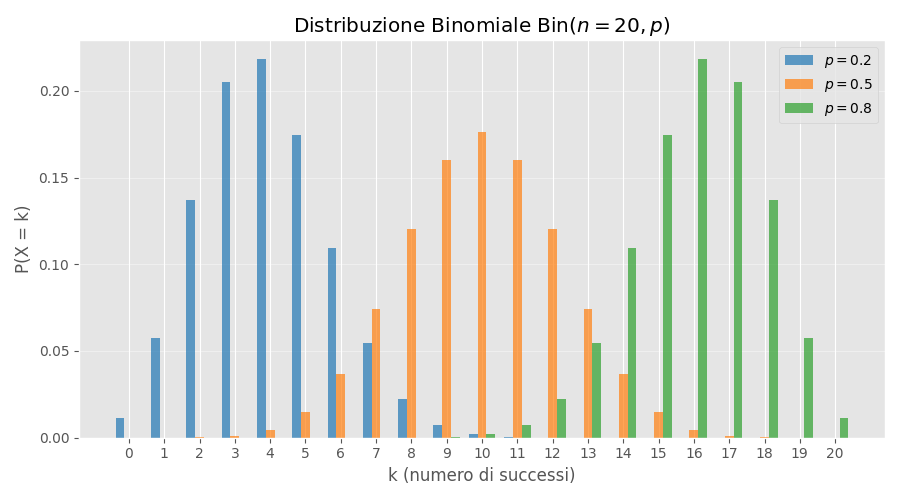
\includegraphics[width=0.8\textwidth]{images/binomiale.png}
    \caption{Esempio di distribuzioni Binomiali con \(n = 20\) e \(p\) variabile.}
    \label{fig:binomiale}
\end{figure}

\subsection{Distribuzione di Poisson}

\begin{definizione}{Distribuzione di Poisson}{poisson}
Una v.a. discreta \(X\) segue una distribuzione di Poisson di parametro \(\nu > 0\), indicata con \(X \sim \text{Pois}(\nu)\), se la sua PMF è:
\[
P(X=k) = \frac{\nu^k e^{-\nu}}{k!}, \quad k=0, 1, 2, \dots \text{}
\]
\end{definizione}

\begin{figure}[H]
    \centering
    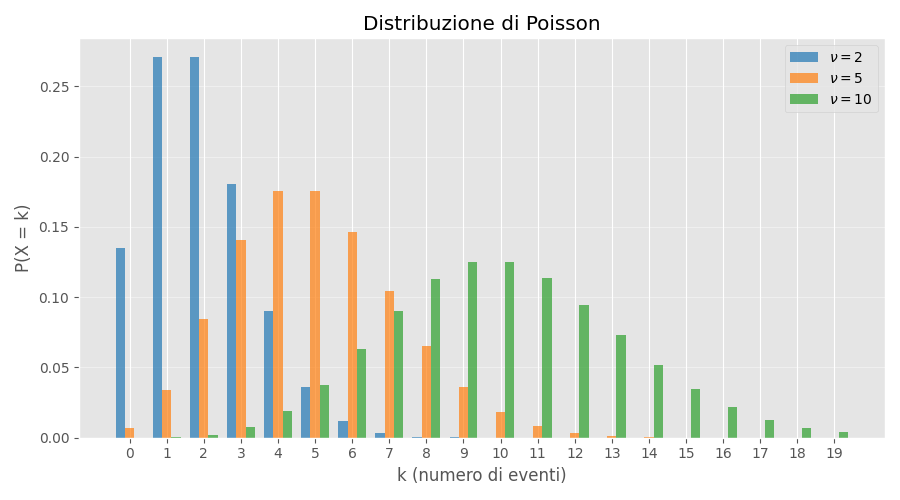
\includegraphics[width=0.8\textwidth]{images/poisson.png}
    \caption{Esempio di distribuzioni di Poisson con \(\nu\) variabile.}
    \label{fig:poisson}
\end{figure}

\begin{nota}{Relazione con la Binomiale}{pois_binom}
La distribuzione di Poisson è il limite della Binomiale per \(n\) grande e \(p\) piccolo. In pratica, se \(p \ll 1\), allora \(\text{Bin}(n,p) \approx \text{Pois}(np)\). Per questo motivo, è usata per contare il numero di successi (eventi rari) in scenari con un gran numero di prove, come il numero di gol in una partita o il numero di iscritti a un corso.

\begin{figure}[H]
    \centering
    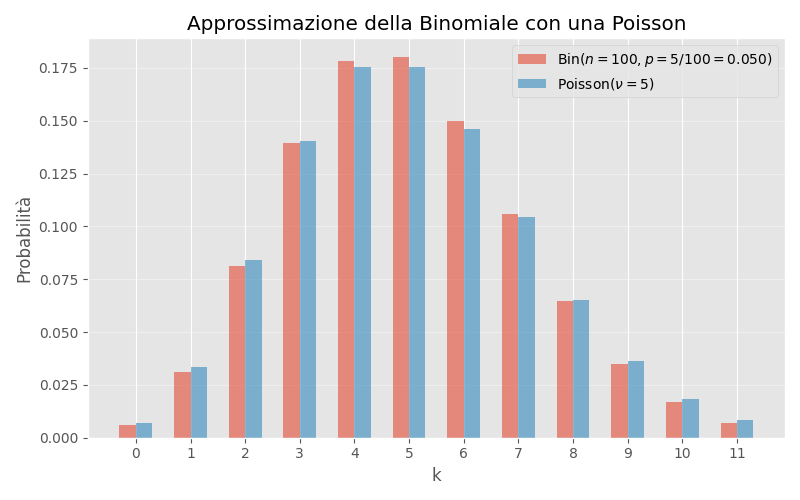
\includegraphics[width=0.8\textwidth]{images/binomiale_vs_poisson.png}
    \caption{Esempio di approssimazione della Binomiale con la Poisson.}
    \label{fig:binomiale_vs_poisson}
\end{figure}

\end{nota}

\begin{proposizione}{Proprietà della Poisson}{pois_props}
\begin{itemize}
    \item \textbf{Riproducibilità:} La somma di v.a. di Poisson indipendenti è ancora una v.a. di Poisson. Se \(X_i \sim \text{Pois}(\nu_i)\) sono indipendenti:
    \[ \sum_{i=1}^{m} X_i \sim \text{Pois}\left(\sum_{i=1}^{m} \nu_i\right) \text{} \]
    \item \textbf{Media e Varianza:} A differenza della Binomiale, media e varianza coincidono.
    \[ E(X) = \nu, \quad \text{Var}(X) = \nu \text{} \]
\end{itemize}
\end{proposizione}

\subsection{Distribuzione Uniforme}

\begin{definizione}{Distribuzione Uniforme Continua}{uniforme}
Una v.a. \(X\) segue una distribuzione Uniforme sull'intervallo \([a,b]\), con \(a<b\) reali, se la sua PDF è costante su quell'intervallo e zero altrove.
\[
f_X(t) = \frac{1}{b-a}, \quad \text{per } a < t < b \text{}
\]
La funzione \texttt{rand()} nei linguaggi di programmazione genera tipicamente campioni da \(\text{Unif}(0,1)\).
\end{definizione}

\begin{proposizione}{Proprietà dell'Uniforme}{unif_props}
\begin{itemize}
    \item \textbf{Media e Varianza:}
    \[ E(X) = \frac{a+b}{2}, \quad \text{Var}(X) = \frac{(b-a)^2}{12} \]
    \item È una classe chiusa per trasformazioni lineari.
\end{itemize}
\end{proposizione}

\begin{figure}[H]
    \centering
    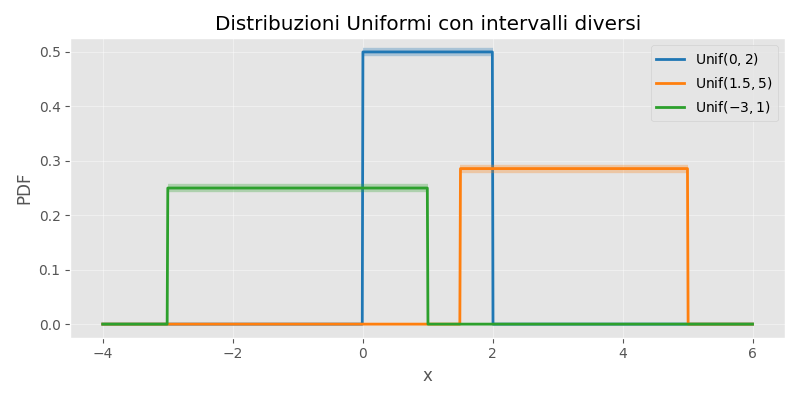
\includegraphics[width=0.8\textwidth]{images/uniforme.png}
    \caption{Esempio di distribuzioni Uniformi con \(a\) e \(b\) variabili.}
    \label{fig:uniforme}
\end{figure}

\subsection{Distribuzione Beta}

\begin{definizione}{Distribuzione Beta}{beta}
Una v.a. \(X\) segue una distribuzione Beta con parametri di forma \(\alpha, \beta > 0\), se la sua PDF è:
\[
f_X(t) = c_p t^{\alpha-1}(1-t)^{\beta-1}, \quad \text{per } 0 < t < 1 \text{}
\]
È una distribuzione molto flessibile, definita su un intervallo limitato.
\end{definizione}

\begin{figure}[H]
    \centering
    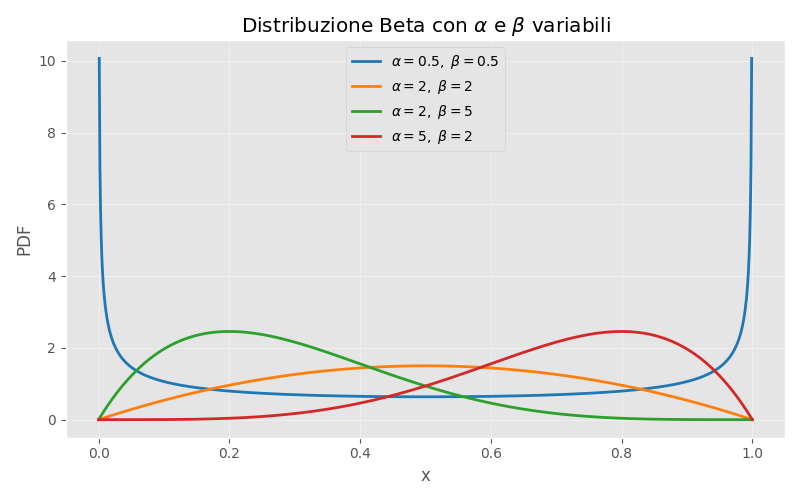
\includegraphics[width=0.8\textwidth]{images/beta.png}
    \caption{Esempio di distribuzioni Beta con \(\alpha\) e \(\beta\) variabili.}
    \label{fig:beta}
\end{figure}

\begin{nota}{Interpretazione della Beta}{beta_interp}
\begin{itemize}
    \item Il caso speciale \(\text{Beta}(1,1)\) corrisponde alla distribuzione \(\text{Unif}(0,1)\).
    \item \textbf{Statistica d'ordine:} La distribuzione \(\text{Beta}(m,n)\) è la distribuzione della \(m\)-esima variabile più piccola tra \(m+n-1\) v.a. \(\text{Unif}(0,1)\) indipendenti.
\end{itemize}
\end{nota}

\subsection{Distribuzione t di Student}

\begin{definizione}{Distribuzione t di Student}{t_student}
La distribuzione t di Student con \(k\) gradi di libertà, \(t(k)\), è definita operativamente dal rapporto tra una v.a. Normale standard e la radice di una Chi-Quadro indipendente, divisa per i suoi gradi di libertà.
Se \(Z \sim \mathcal{N}(0,1)\) e \(W \sim \chi^2(k)\) sono indipendenti, allora:
\[
T = \frac{Z}{\sqrt{W/k}} \sim t(k) \text{}
\]
\end{definizione}

\begin{proposizione}{Proprietà della t di Student}{t_props}
\begin{itemize}
    \item Ha una forma a campana simile alla Normale, ma con code più "pesanti".
    \item Per \(k \to \infty\), la distribuzione \(t(k)\) converge alla Normale standard \(\mathcal{N}(0,1)\).
    \item La media è \(E(T)=0\) (per \(k>1\)).
\end{itemize}
\end{proposizione}

\begin{figure}[H]
    \centering
    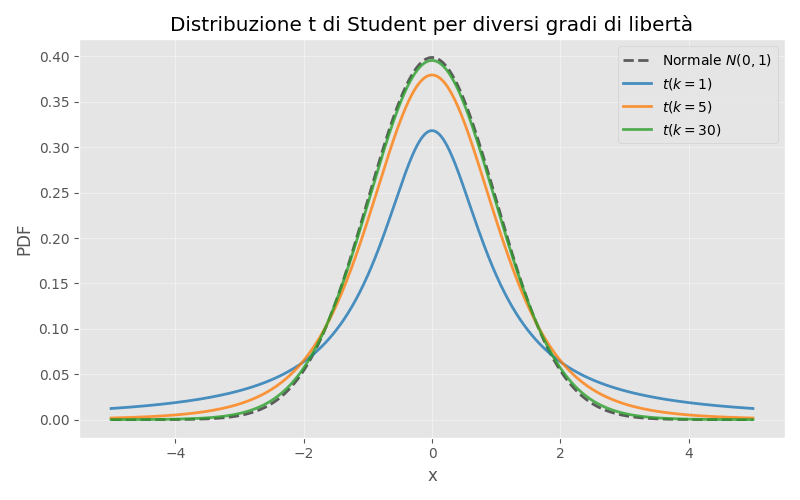
\includegraphics[width=0.8\textwidth]{images/t_student.png}
    \caption{Esempio di distribuzioni t di Student con \(k\) variabile.}
    \label{fig:t_student}
\end{figure}

\subsection{Distribuzione F di Fisher}

\begin{definizione}{Distribuzione F di Fisher}{f_fisher}
La distribuzione F di Fisher con \((m, n)\) gradi di libertà, \(F(m,n)\), è definita operativamente come il rapporto tra due v.a. Chi-Quadro indipendenti, ciascuna divisa per i propri gradi di libertà.
Se \(W_1 \sim \chi^2(m)\) e \(W_2 \sim \chi^2(n)\) sono indipendenti, allora:
\[
F = \frac{W_1/m}{W_2/n} \sim F(m,n) \text{}
\]
\end{definizione}

\begin{figure}[H]
    \centering
    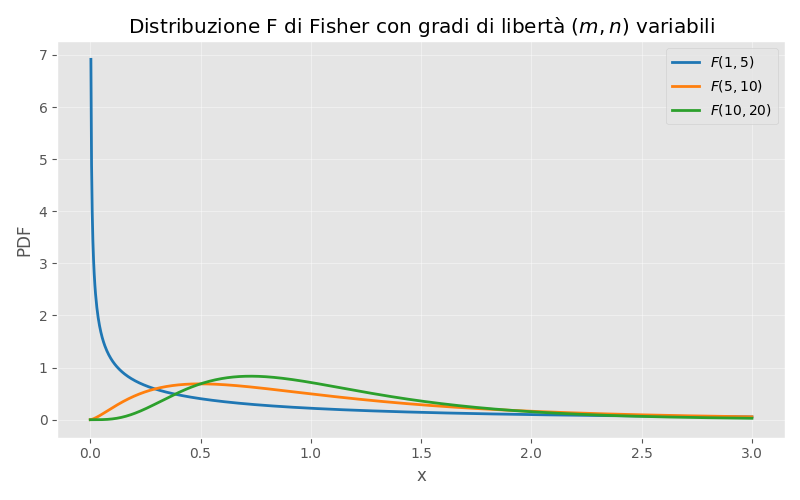
\includegraphics[width=0.8\textwidth]{images/f_fisher.png}
    \caption{Esempio di distribuzioni F di Fisher con \((m,n)\) variabili.}
    \label{fig:f_fisher}
\end{figure}

\begin{nota}{Uso della Distribuzione F}{f_uso}
È usata principalmente per confrontare due varianze campionarie. I parametri \(m\) e \(n\) sono i gradi di libertà del numeratore e del denominatore, rispettivamente.
\end{nota}

\subsection{Distribuzione Uniforme Discreta}

\begin{definizione}{Distribuzione Uniforme Discreta}{unif_discreta}
Una v.a. \(X\) segue una distribuzione Uniforme Discreta se può assumere \(n\) valori, \(\{1, 2, \dots, n\}\), ciascuno con la stessa probabilità. L'esempio classico è il lancio di un dado a \(n\) facce.
\[
P(X = i) = \frac{1}{n}, \quad \text{per } i=1, 2, \dots, n
\]
\end{definizione}

\begin{figure}[H]
    \centering
    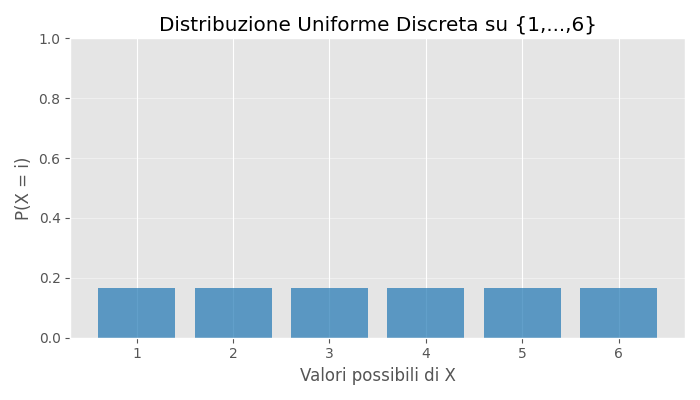
\includegraphics[width=0.8\textwidth]{images/uniforme_discreta.png}
    \caption{Esempio di distribuzioni Uniformi Discrete su \(\{1, 2, \dots, 6\}\).}
    \label{fig:uniforme_discreta}
\end{figure}

\begin{proposizione}{Proprietà dell'Uniforme Discreta}{unif_discreta_props}
\begin{itemize}
    \item \textbf{Non è riproducibile:} La somma di due o più v.a. uniformi discrete indipendenti non è più uniforme. La sua distribuzione tende a una forma a campana (analogo discreto del TLC).
    \item \textbf{Media e Varianza:}
    \[ E(X) = \frac{n+1}{2}, \quad \text{Var}(X) = \frac{n^2-1}{12} \]
\end{itemize}
\end{proposizione}

\subsection{Processo di Bernoulli e Distribuzioni Associate}
Molte distribuzioni discrete di base emergono dal \textbf{Processo di Bernoulli}, l'analogo a tempo discreto del Processo di Poisson.

\begin{definizione}{Processo di Bernoulli}{proc_bernoulli}
Un processo di Bernoulli è una sequenza di prove o esperimenti indipendenti, ciascuno con due soli esiti possibili: "successo" (con probabilità \(p\)) o "insuccesso" (con probabilità \(1-p\)).
\end{definizione}

\begin{nota}{Variabili aleatorie in un Processo di Bernoulli}{vars_bernoulli}
All'interno di un processo di Bernoulli si possono definire diverse variabili aleatorie di interesse:
\begin{itemize}
    \item \textbf{Numero di successi \(N_n\):} Il conteggio dei successi in \(n\) prove. Segue una distribuzione \(\text{Bin}(n,p)\).
    \item \textbf{Tempo del primo successo \(T_1\):} Il numero di prove necessarie per ottenere il primo successo. Segue una distribuzione \(\text{Geom}(p)\).
    \item \textbf{Tempo dell'm-esimo successo \(S_m\):} Il numero di prove necessarie per ottenere l'\(m\)-esimo successo. Segue una distribuzione \(\text{NegBin}(m,p)\).
\end{itemize}
\end{nota}

\subsection{Distribuzione Geometrica}

\begin{definizione}{Distribuzione Geometrica}{geometrica}
Una v.a. \(X\) segue una distribuzione Geometrica di parametro \(p \in (0,1]\) se la sua PMF è:
\[
P(X=k) = p(1-p)^{k-1}, \quad k=1, 2, 3, \dots
\]
Rappresenta il numero di prove necessarie per ottenere il primo successo in un processo di Bernoulli.
\end{definizione}

\begin{figure}[H]
    \centering
    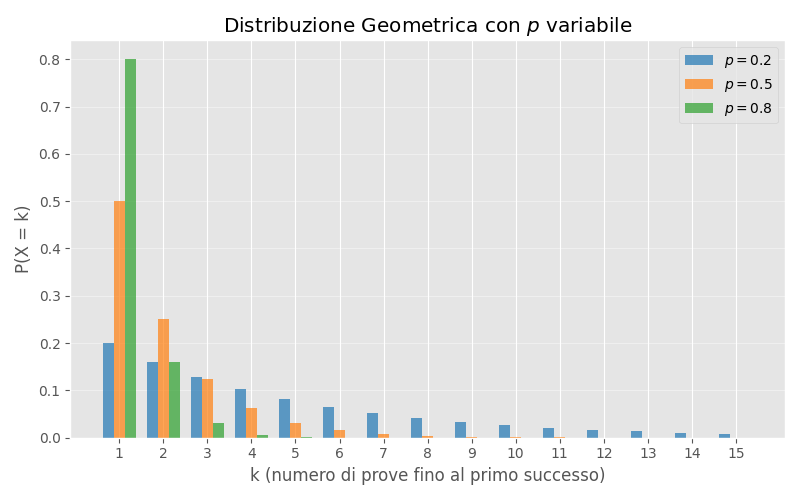
\includegraphics[width=0.8\textwidth]{images/geometrica.png}
    \caption{Esempio di distribuzioni Geometriche con \(p\) variabile.}
    \label{fig:geometrica}
\end{figure}

\begin{proposizione}{Proprietà della Geometrica}{geom_props}
\begin{itemize}
    \item È la versione discreta della distribuzione Esponenziale.
    \item \textbf{Media e Varianza:}
    \[ E(X) = \frac{1}{p}, \quad \text{Var}(X) = \frac{1-p}{p^2} \]
\end{itemize}
\end{proposizione}

\subsection{Distribuzione Binomiale Negativa}
Questa distribuzione generalizza la Geometrica al caso di \(r\) successi.

\begin{definizione}{Distribuzione Binomiale Negativa}{negbin}
Esistono due definizioni comuni per la Binomiale Negativa \(\text{NegBin}(r,p)\):
\begin{enumerate}
    \item \textbf{Numero di prove:} \(X\) è il numero totale di prove per ottenere \(r\) successi. La sua PMF è:
    \[ P(X=k) = \binom{k-1}{r-1}p^r(1-p)^{k-r}, \quad k=r, r+1, \dots \]
    \item \textbf{Numero di insuccessi:} \(\tilde{X}\) è il numero di insuccessi che avvengono prima di ottenere \(r\) successi. La sua PMF, usata spesso in software come SciPy, è:
    \[ P(\tilde{X}=k) = \binom{k+r-1}{k}p^r(1-p)^{k}, \quad k=0, 1, 2, \dots \]
\end{enumerate}
\end{definizione}

\begin{figure}[H]
    \centering
    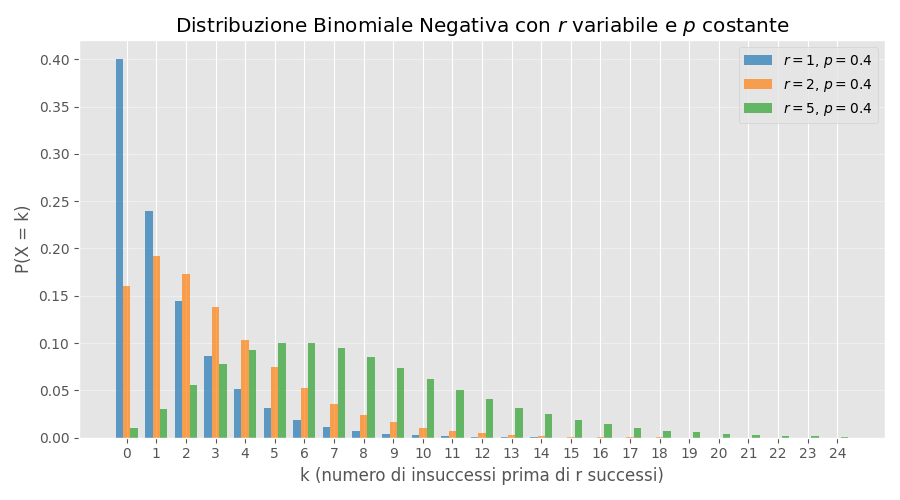
\includegraphics[width=0.8\textwidth]{images/negbin.png}
    \caption{Esempio di distribuzioni Binomiali Negative con \(r\) variabile e \(p\) costante per numero di insuccessi.}
    \label{fig:negbin}
\end{figure}


\begin{figure}[H]
    \centering
    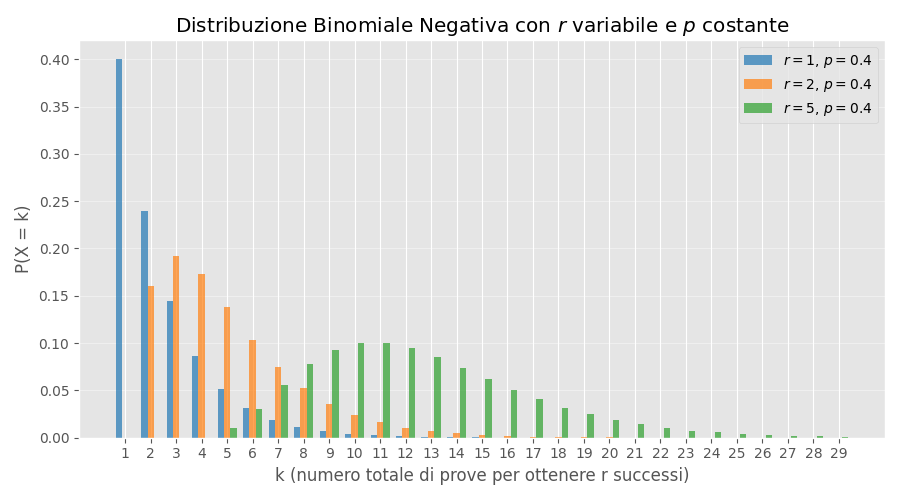
\includegraphics[width=0.8\textwidth]{images/negbin_trials.png}
    \caption{Esempio di distribuzioni Binomiali Negative con \(r\) variabile e \(p\) costante per numero di prove.}
    \label{fig:negbin_trials}
\end{figure}

\begin{proposizione}{Proprietà della Binomiale Negativa}{negbin_props}
\begin{itemize}
    \item Se \(r=1\), si ottiene la distribuzione Geometrica.
    \item \textbf{Riproducibilità:} La somma di v.a. Binomiali Negative indipendenti con lo stesso \(p\) è ancora una Binomiale Negativa. Se \(X_i \sim \text{NegBin}(r_i, p)\) sono indipendenti:
    \[ \sum X_i \sim \text{NegBin}\left(\sum r_i, p\right) \]
    \item \textbf{Media e Varianza (per la def. 1):}
    \[ E(X) = \frac{r}{p}, \quad \text{Var}(X) = \frac{r(1-p)}{p^2} \]
\end{itemize}
\end{proposizione}
